\documentclass[ignorenonframetext,10pt,aspectratio=169]{beamer}

\usepackage{umut}
\usepackage{umuttr}
\usepackage{usynsem}
\usepackage[utf8]{inputenc}
\usepackage{uling}
\usepackage{natbib,unatbib}
\usepackage{linguex}
         \renewcommand{\refdash}{}
\usepackage{ubeamer}
\usepackage{verbatim}
\usepackage{adjustbox}
\usepackage{fancyvrb}

\usepackage{tikz-qtree}
\usetikzlibrary{er,positioning}

\title{C-command and binding}
\author{\  \\  {\it Based on Koeneman \& Zeiljstra (2017)} \\ \vspace{20pt} Umut \"Ozge\\  }

\date{COGS 532: Theoretical Linguistics\\ METU, Informatics}

\begin{document}

\begin{frame}\frametitle{}
\thispagestyle{empty}
\maketitle
\end{frame}

\begin{frame}[t,plain]{Domain of binding}

		\bigskip

		\ex. \colb{John} said that \colg{Peter} thought that \colr{Harry} blamed himself.

		\bigskip

		\ex. \colb{John} said that \colg{Peter} thought that \colr{Harry} blamed him.

		\bigskip

		\ex. John wants \lbrac{\alert{FinP}}{himself to succeed}. 

		\bigskip

		\ex. We expected \lbrac{\alert{FinP}}{ourselves to do better next time}. 

\end{frame}


\begin{frame}[t,plain]{Dominance}

		\bigskip

		A node $A$ \alert{dominates} a node $B$ if and only if you can reach from $A$ to $B$ by going \alert{only down} in the tree. 

		\bigskip


		A node $A$ \alert{immediately dominates} a node $B$ if and only if you can reach from $A$ to $B$ by going \alert{one step down} in the tree. 

\end{frame}

\begin{frame}[t,plain]{Binding conditions revised}
		\bigskip
		\bigskip
		\bigskip

		\colb{Principle A:}

		A reflexive must be bound within the closest \alert{finite} FinP dominating it.

		\bigskip

		\colb{Principle B:}

		A non-reflexive pronoun cannot be bound within the closest \alert{finite} FinP dominating it.

\end{frame}

\begin{frame}[t,plain]{}
\ex. John said that Peter thought that Harry blamed himself.

\begin{center}
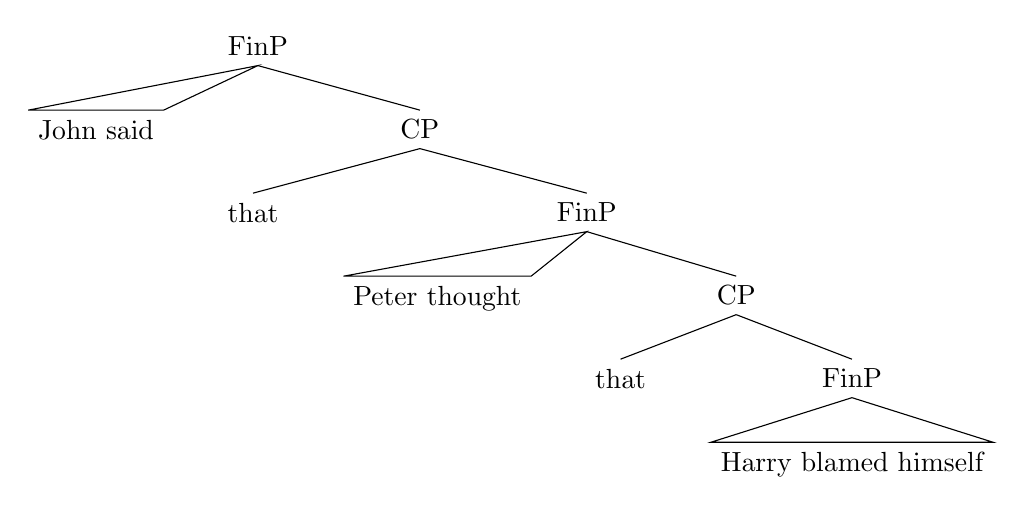
\begin{tikzpicture}
\tikzset{level distance=30pt, sibling distance=20pt}
\tikzset{every tree node/.style={align=center,anchor=north}}
		\Tree[.{FinP} \edge[roof]; {John said}  [.{CP} that [.{FinP} \edge[roof]; {Peter thought} [.{CP} that [.{FinP} \edge[roof]; {Harry blamed himself} ] ] ] ] ] 
\end{tikzpicture}
\end{center}
\end{frame}

\begin{frame}[t,plain]{}
\ex. John said that Peter thought that Harry blamed him.

\begin{center}
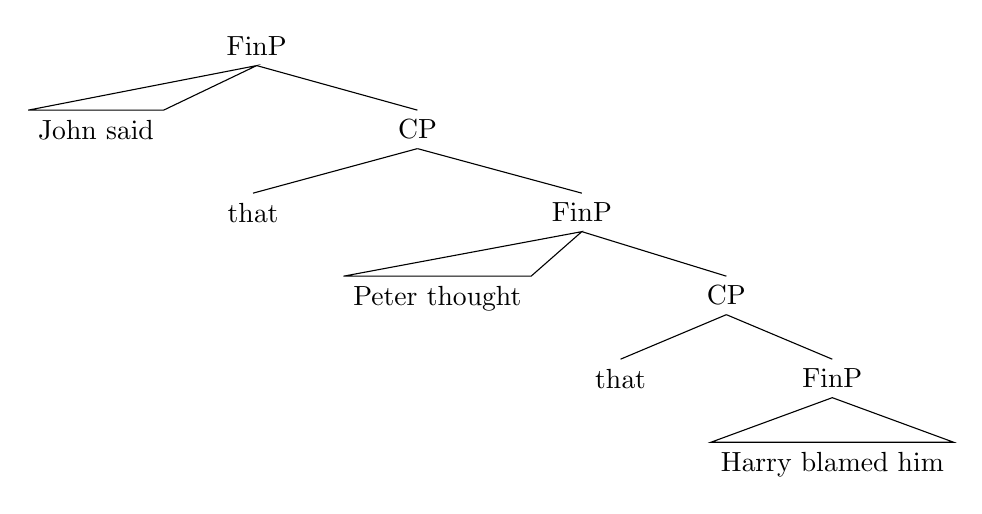
\begin{tikzpicture}
\tikzset{level distance=30pt, sibling distance=20pt}
\tikzset{every tree node/.style={align=center,anchor=north}}
		\Tree[.{FinP} \edge[roof]; {John said}  [.{CP} that [.{FinP} \edge[roof]; {Peter thought} [.{CP} that [.{FinP} \edge[roof]; {Harry blamed him} ] ] ] ] ] 
\end{tikzpicture}
\end{center}
\end{frame}

\begin{frame}[t,plain]{Problems}

\bigskip

		\ex. \a. *The book about the president\ind{i} upset himself\ind{i}.
		\b. *John\ind{i}'s sister likes himself\ind{i}.
		\b. *Admiring Mary\ind{i} pleases herself\ind{i}.

\begin{center}
		\footnotesize
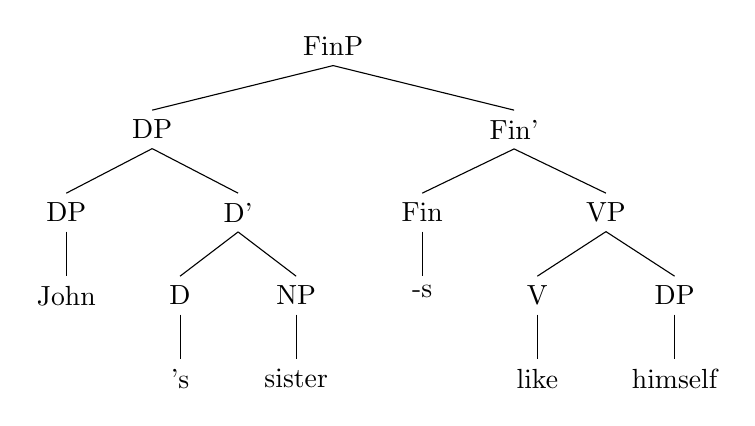
\begin{tikzpicture}
\tikzset{level distance=30pt, sibling distance=20pt}
\tikzset{every tree node/.style={align=center,anchor=north}}
\Tree[.{FinP} [.{DP} [.{DP} John ] [.{D'} [.{D} 's ] [.{NP} sister ] ] ] [.{Fin'} [.{Fin} -s ] [.{VP} [.{V} like ] [.{DP} himself ] ] ] ] 
\end{tikzpicture}
\end{center}
\end{frame}
\end{frame}

\begin{frame}[t,plain]{C-command}
\bigskip
\bigskip

$A$ c-commands $B$ if and only if the node that immediately dominates $A$ dominates $B$ and $A$ does not dominate $B$.

\bigskip
{\scriptsize
\adjustbox{valign=t}{
\begin{tikzpicture}
\tikzset{level distance=30pt, sibling distance=20pt}
\tikzset{every tree node/.style={align=center,anchor=north}}
\Tree[.{XP} A [.{X'} X [.{YP} ... B ] ] ] 
\end{tikzpicture}}
\adjustbox{valign=t}{
\begin{tikzpicture}
\tikzset{level distance=30pt, sibling distance=20pt}
\tikzset{every tree node/.style={align=center,anchor=north}}
\Tree[.{XP} [.{ZP} Z A ] [.{X'} X [.{YP} ... B ] ] ] 
\end{tikzpicture}}
\adjustbox{valign=t}{
\begin{tikzpicture}
\tikzset{level distance=30pt, sibling distance=20pt}
\tikzset{every tree node/.style={align=center,anchor=north}}
\Tree[.{XP} [.{ZP} Z K ] [.{A} X [.{YP} ... B ] ] ] 
\end{tikzpicture}}
\adjustbox{valign=t}{
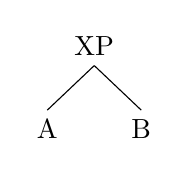
\begin{tikzpicture}
\tikzset{level distance=30pt, sibling distance=20pt}
\tikzset{every tree node/.style={align=center,anchor=north}}
\Tree[.{XP} A B ] 
\end{tikzpicture}}
}
\end{frame}

\begin{frame}[t,plain]{Binding conditions revised}
		\bigskip

		\colb{Principle A:}

		A reflexive must be bound by a c-commanding antecedent, where the  antecedent is dominated by the closest finite FinP that dominates the reflexive.

		\bigskip

		\colb{Principle B:}

		A non-reflexive pronoun cannot be bound by a c-commanding antecedent, where the  antecedent is dominated by the closest finite FinP that dominates the reflexive.

\end{frame}

\begin{frame}[t,plain]{C-command failure}

\bigskip

		\ex. *John\ind{i}'s sister likes himself\ind{i}.

\begin{center}
		\footnotesize
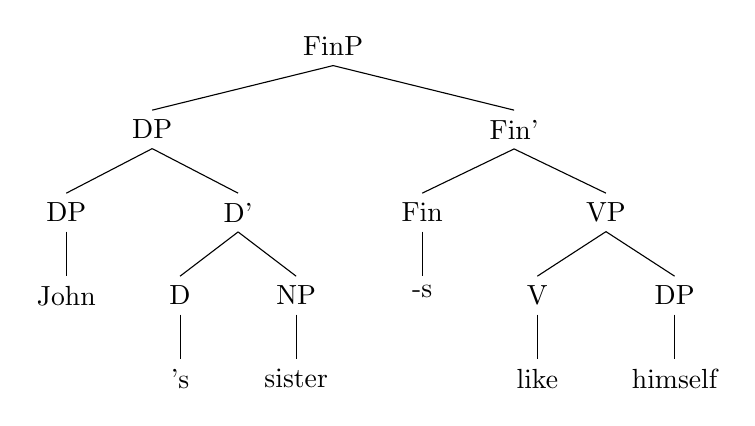
\begin{tikzpicture}
\tikzset{level distance=30pt, sibling distance=20pt}
\tikzset{every tree node/.style={align=center,anchor=north}}
\Tree[.{FinP} [.{DP} [.{DP} John ] [.{D'} [.{D} 's ] [.{NP} sister ] ] ] [.{Fin'} [.{Fin} -s ] [.{VP} [.{V} like ] [.{DP} himself ] ] ] ] 
\end{tikzpicture}
\end{center}
\end{frame}
\end{frame}

\begin{frame}[t,plain]{``Closest FinP'' (locality) failure}
		\ex. *John said that Peter\ind{i} thought that Harry blamed himself\ind{i}.

\begin{center}
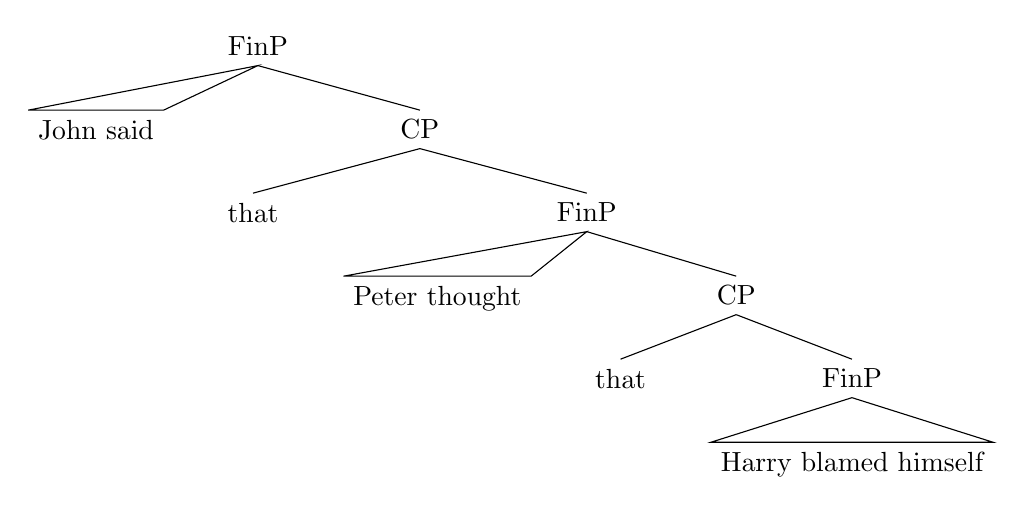
\begin{tikzpicture}
\tikzset{level distance=30pt, sibling distance=20pt}
\tikzset{every tree node/.style={align=center,anchor=north}}
		\Tree[.{FinP} \edge[roof]; {John said}  [.{CP} that [.{FinP} \edge[roof]; {Peter thought} [.{CP} that [.{FinP} \edge[roof]; {Harry blamed himself} ] ] ] ] ] 
\end{tikzpicture}
\end{center}
\end{frame}

\begin{frame}[t,plain]{Binding in other phrases}

		\ex. John likes Mary\ind{i}'s ideas about herself\ind{i}.

\begin{center}
{\scriptsize
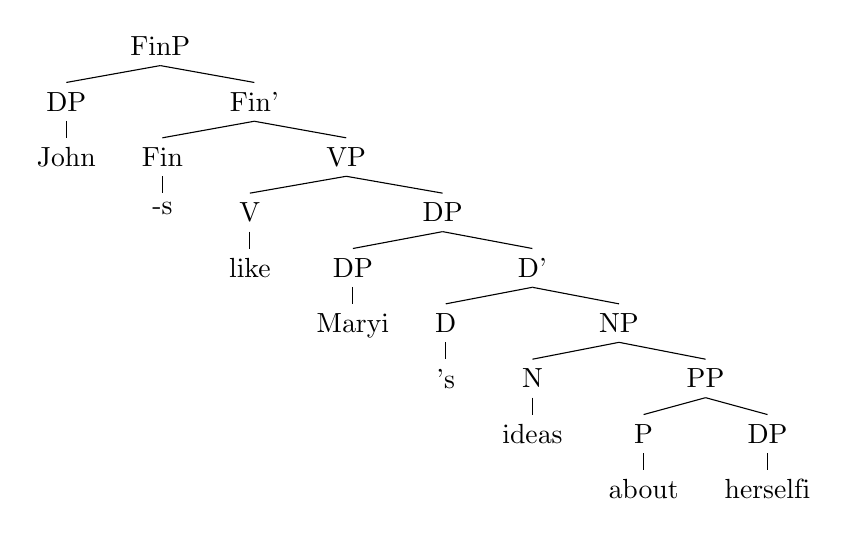
\begin{tikzpicture}
\tikzset{level distance=20pt, sibling distance=10pt}
\tikzset{every tree node/.style={align=center,anchor=north}}
\Tree[.{FinP} [.{DP} John ] [.{Fin'} [.{Fin} -s ] [.{VP} [.{V} like ] [.{DP} [.{DP} Mary\ind{i} ] [.{D'} [.{D} 's ] [.{NP} [.{N} ideas ] [.{PP} [.{P} about ] [.{DP} herself\ind{i} ] ] ] ] ] ] ] ] 
\end{tikzpicture}
}
\end{center}
\end{frame}

\begin{frame}[t,plain]{}

\end{frame}

\begin{frame}[t,plain]{}

\end{frame}

\begin{frame}[t,plain]{} 
\end{frame}

\begin{frame}[t,plain]{}

\end{frame}

\begin{frame}[t,plain]{}

\end{frame}

\begin{frame}[t,plain]{}

\end{frame}

\begin{frame}[t,plain]{}

\end{frame}

\begin{frame}[t,plain]{}

\end{frame}

\begin{frame}[t,plain]{}

\end{frame}

\begin{frame}[t,plain]{}

\end{frame}

\end{document}
